\documentclass[a4paper,10pt]{ctexart}
%引用设置使用Bibtex
\usepackage{gbt7714}
\bibliographystyle{gbt7714-numerical}
%页面设置
\usepackage{geometry}
%字体设置
\usepackage{fontspec}
%\setmainfont{Times New Roman}
%定理环境
\usepackage{amsmath}
\numberwithin{equation}{section}
\usepackage{amsthm}
\newtheorem*{definition}{Definition}
\newtheorem{theorem}{Theorem}
\newtheorem{lemma}{Lemma}
\newtheorem*{corollary}{Corollary}
\newtheorem*{proposition}{Proposition}
\newtheorem*{example}{Example}
%数学环境字体
\usepackage{bm}
\usepackage[all]{xy}
%加载 TikZ 用于绘制交换图
\usepackage{tikz-cd}
\usepackage{tikz}
\usepackage{pgfplots}
\newcommand{\tikzdef}{\pgfmathsetmacro} % 在tikzpicture内的foreach循环中定义实数临时变量
%颜色
\usepackage{color,xcolor}

\definecolor{miku}{RGB}{57,197,187}
\definecolor{sakura}{RGB}{255,192,203}
\definecolor{rose}{RGB}{255,228,225}
\definecolor{brown}{RGB}{210,105,30}
\definecolor{lbrown}{RGB}{239,235,224}
\definecolor{bule}{RGB}{0,47,167}
\definecolor{lyellow}{RGB}{250,250,210}
\definecolor{lpurple}{RGB}{255,240,245}
\definecolor{lbule}{RGB}{135,206,250}
\definecolor{gbule}{RGB}{64,224,208}
\definecolor{green}{RGB}{138,200,207}
\definecolor{lgreen}{RGB}{225,255,255}
\definecolor{lorange}{RGB}{248,172,140}
\definecolor{salmon}{RGB}{250,128,114}
\definecolor{burgundy}{rgb}{0.5, 0.0, 0.13}
%链接设置
\usepackage[colorlinks=true,pdfstartview=FitH,linkcolor=blue,anchorcolor=violet, citecolor=magenta]{hyperref} 
%封面
\usepackage{pdfpages}
\usepackage{mathrsfs}
\usepackage{amssymb}
\usepackage{graphicx}
\usepackage{lipsum}
%彩色框
\usepackage{framed}
\usepackage{tcolorbox}
\tcbuselibrary{breakable}
\tcbuselibrary{theorems}
\tcbuselibrary{skins}
\usepackage{colortbl}
\usepackage{float}
\usepackage[export]{adjustbox}
\newtcolorbox[auto counter,number within=section]{notebox}[2][]{%
colback=miku!2!white,
colframe=miku,
coltitle=white,
fonttitle=\bfseries,
rightrule=2pt,
leftrule=2pt,
bottomrule=2pt,
colbacktitle=miku,
theorem style=standard,
breakable,
arc=2pt,
drop fuzzy shadow=black!20!white,
title=Note~\thetcbcounter: #2,#1}
\newtcolorbox[auto counter,number within=section]{markbox}[2][]{%
colback=miku!2!white,
colframe=miku,
coltitle=white,
fonttitle=\bfseries,
rightrule=0pt,
leftrule=0pt,
bottomrule=2pt,
colbacktitle=miku,
theorem style=standard,
breakable,
arc=0pt,
drop fuzzy shadow=black!20!white,
title=Remark~\thetcbcounter: #2,#1}
\newtcolorbox[no counter]{theorems}[2][]{%
width=12cm,
center,
sidebyside,
sidebyside adapt=left,
sidebyside gap=6mm,
sidebyside align=center seam,
colback=burgundy!2!white,
colframe=burgundy,
coltitle=white,
fonttitle=\bfseries,
rightrule=1pt,
leftrule=1pt,
bottomrule=2pt,
colbacktitle=burgundy,
theorem style=standard,
enhanced,
drop fuzzy shadow southeast=black!30!white,
breakable,
arc=0pt,
title=Theorem. #2,#1}
\newtcolorbox[no counter]{definitions}[2][]{%
width=12cm,
center,
colback=lyellow!2!white,
colframe=yellow!3!lyellow,
coltitle=bule,
fonttitle=\bfseries,
rightrule=0pt,
leftrule=1pt,
bottomrule=2pt,
colbacktitle=lyellow,
theorem style=standard,
breakable,
arc=5pt,
enhanced,
drop fuzzy shadow southeast=black!20!white,
title=Definition. #2,#1}
\newtcolorbox[auto counter,number within=section]{corollarys}[2][]{%
colback=lyellow!2!white,
colframe=lyellow,
coltitle=bule,
fonttitle=\bfseries,
rightrule=0pt,
leftrule=1pt,
bottomrule=2pt,
colbacktitle=lyellow,
theorem style=standard,
breakable,
arc=0pt,
enhanced,
drop fuzzy shadow southeast=black!20!white,
title=Corollary~\thetcbcounter: #2,#1}
\newtcolorbox[auto counter,number within=section]{lemmas}[2][]{%
width=12cm,
center,
colback=lyellow!2!white,
colframe=lorange!30!sakura,
coltitle=bule,
fonttitle=\bfseries,
rightrule=0pt,
leftrule=1pt,
bottomrule=2pt,
colbacktitle=lorange!30!sakura,
theorem style=standard,
breakable,
arc=5pt,
enhanced,
drop fuzzy shadow southeast=black!20!white,
title=Lemma. #2,#1}
\newtcolorbox[auto counter,number within=section]{propositions}[2][]{%
width=12cm,
center,
colback=salmon!5,
colframe=salmon!90!black,
coltitle=white,
fonttitle=\bfseries,
rightrule=1pt,
leftrule=1pt,
bottomrule=2pt,
colbacktitle=salmon!90!black,
theorem style=standard,
breakable,
arc=5pt,
enhanced,
drop fuzzy shadow southeast=black!20!white,
title=Proposition. #2,#1}
\newtcolorbox[no counter]{egbox}[2][]{%
width=12cm,
center,
colback=black!5!white,
colframe=black!20!white,
coltitle=black,
fonttitle=\bfseries,
rightrule=1pt,
leftrule=1pt,
bottomrule=2pt,
colbacktitle=black!20!white,
theorem style=standard,
breakable,
arc=0pt,
enhanced,
drop fuzzy shadow southeast=black!20!white,
title=Example. #2,#1}

%\begin{figure}[H]
%\centering
%\includegraphics[center]{pic.png}
%\end{figure}
\geometry{left=3cm,right=3cm,top=2cm,bottom=2cm}
\tcbuselibrary{most}

\usepackage[linesnumbered,ruled,vlined]{algorithm2e}
\usepackage{algorithmic}

\SetKwProg{Fn}{function}{\string:}{}
\newcommand{\forcond}{$i=0$ \KwTo $n$}
\SetKwFunction{FRecurs}{FnRecursive}
\SetKwInput{KwCost}{Cost}

\usepackage{holtpolt}

%自定义设置
\renewcommand{\proofname}{Proof.}
\renewcommand{\contentsname}{ Content }
\newcommand{\image}[2]{
    \centering
    \includegraphics[width={#1}\textwidth]{#2}
}



\newcommand\keywords[1]{\vskip2ex\par\noindent\normalfont{\textbf{关键词}: #1}}
\newcommand{\ekeywords}[1]{\vskip2ex\par\noindent\normalfont{\bfseries Key Words: }#1}
\newcommand{\miku}{\textcolor{miku}}
\newcommand{\sakura}{\textcolor{sakura}}
\newcommand{\brown}{\textcolor{brow}}
\newcommand{\red}{\textcolor{red}}
\newcommand{\blue}{\textcolor{blue}}
\newcommand{\A}{\mathcal{A}}
\newcommand{\C}{\mathbb{C}}
\newcommand{\al}{\alpha}
\newcommand{\sa}{$\sigma$-algebra}
\newcommand{\Bsa}{Borel $\sigma$-algebra}
\newcommand{\F}{\mathcal{F}}
\newcommand{\N}{\mathcal{N}}
\newcommand{\M}{\mathcal{M}}
\newcommand{\m}{ $\mathcal{M}$ }
\newcommand{\B}{\mathcal{B}}
\newcommand{\myP}{\mathcal{P}}
\renewcommand{\bf}[1]{\textbf{#1}}

\newcommand{\myRom}[1]{\uppercase\expandafter{\romannumeral#1}}
\newcommand{\pl}{$ L^p(X) $}
\newcommand{\twol}{$ L^2(X) $}

\usepackage{booktabs}

\begin{document}
\hfill\vbox{\hbox{Numerical Analysis}\hbox{陈曦,UESTC}\hbox{Summer, 2024}}

\begin{center}\Large
    \textbf{数值线性代数}\\{\normalsize\bf {线性方程组的直接解法}}
\end{center}
\vskip 30pt
\small {参考书目:
\begin{itemize}
    \item Accuracy and Stability of Numerical Algorithms(Higham,2002)
    \item Fundamentals of Matrix Computations(Watkins,2010)
    \item 数值线性代数(徐树方,2013)
\end{itemize}}

本文主要介绍线性方程组的直接解法,即在没有舍入误差的情况下经过有限次运算可以求得线性系统的精确解的方法,故直接法又被称作精确法。通常,可以根据系数矩阵的性质来选择合适的直接法。矩阵的稀疏性以及相关算法在本文没有详细介绍,因为对于大型稀疏矩阵,迭代法在绝大多数情况下是比直接法更好的选择。一般地,一个合适的算法应当满足:
\begin{enumerate}
    \item 问题有解时给出解,无解时给出无解的信息;
    \item 可以检测出各种异常情况,如除零、矩阵奇异等;
    \item 尽可能地高效和准确稳定。
\end{enumerate}
在设计算法时,需要尽量满足以上要求。另外,考虑到计算机自身的存储结构特点,我们在计算时希望尽可能地使用(分块)矩阵运算来代替分量运算,以提高计算效率。

\begin{quotation}
    现代计算机大都采用多级储存的方式,主要的部件有:寄存器(Register)、缓冲器(Cache)、主存(Memory)、磁盘(Disk)和磁带(Tape)。其中计算单元直接与寄存器相连并交换信息,计算时需将所需的数据逐级传递到寄存器,而计算结束之后需要再将寄存器内的数据再逐级传递出去。从寄存器依次到磁带其处理传递信息的速度越来越慢,一般具有量级上的差异,造价也是随着级别的下降而下降,寄存器非常昂贵,而磁盘和磁带则非常便宜,所以一般计算机的磁盘和磁带的容量都很大,而缓冲器和寄存器的容量就很小。因此,为了提高计算机的运算速度,在编制软件时,需要尽可能地减少内外存及寄存器和主存之间地数据传递。
\end{quotation}

\begin{figure}[htpb]
    \centering
    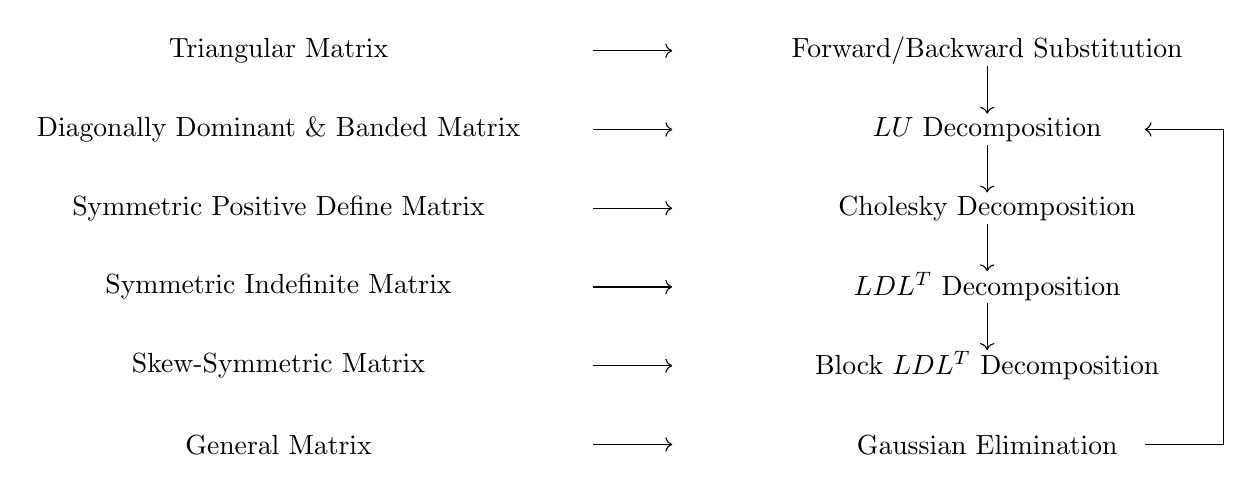
\begin{tikzpicture}
        \node at (0, 2) {Diagonally Dominant \& Banded Matrix};
        \node at (0, 3) {Triangular Matrix};
        \node at (0, 1) {Symmetric Positive Define Matrix};
        \node at (0, 0) {Symmetric Indefinite Matrix};
        \node at (0, -1) {Skew-Symmetric Matrix};
        \node at (0, -2) {General Matrix};
        \draw[->] (4, 2) -- (5, 2); \node at (9, 2) {$ LU $ Decomposition};
        \draw[->] (4, 3) -- (5, 3); \node at (9, 3) {Forward/Backward Substitution};
        \draw[->] (4, 1) -- (5, 1); \node at (9, 1) {Cholesky Decomposition};
        \draw[->] (4, 0) -- (5, 0); \node at (9, 0) {$ LDL^T $ Decomposition};
        \draw[->] (4, -1) -- (5, -1); \node at (9, -1) {Block $ LDL^T $ Decomposition};
        \draw[->] (4, -2) -- (5, -2); \node at (9, -2) {Gaussian Elimination};
        \draw[->] (9, 2.8) -- (9, 2.2);
        \draw[->] (9, 1.8) -- (9, 1.2);
        \draw[->] (9, 0.8) -- (9, 0.2);
        \draw[->] (9, -0.2) -- (9, -0.8);
        \draw[->] (11, -2) -- (12, -2) -- (12, 2) -- (11, 2);
      \end{tikzpicture}
    \caption{矩阵性质与相应方法}
    \label{fig:PropertyMethod}
\end{figure}
本文将先介绍最通用也最基础的高斯消元法,之后按从图\ref{fig:PropertyMethod}的上方到下方的顺序介绍这些方法,越上面的矩阵性质越好,对应的方法也越高效,但是适用性也越窄。在介绍每个方法时,将给出伪代码及其算法实现,并研究算法复杂度和稳定性。

\section{三角矩阵的直接解法}
这一节需要求解的问题形如$ Ux=b $,其中
\[
    U = \begin{pmatrix}
        u_{11} & u_{12} & \cdots & u_{1n} \\
        0 & u_{22} & \cdots & u_{2n} \\
        \vdots & \vdots & \ddots & \vdots \\
        0 & 0 & \cdots & u_{nn}
    \end{pmatrix}
\]
是任意的对角元非零上三角矩阵。
\subsection{后代法}
注意到解向量$ x $的第$ i $个分量$ x_i $满足
\[
    x_i = \frac{b_i - \sum_{j=i+1}^{n} u_{ij}x_j}{u_{ii}},
\]
在计算$ x_i $时只需要后$ n-i $个分量,而$ x_n = b_n / u_{nn} $,因此我们可以按照从后到前的顺序逐个计算$ x_i $。因为在计算每个$ x_i $时需要使用到$ U $的第$ i $行(row-oriented),因此这种方法称为\emph{行向}后代法,另外由于上式中的$ \sum_{j=i+1}^{n} u_{ij}x_j $可视作内积,因此该方法也称作\emph{内积型}(inner-product form)后代法。伪代码如算法\ref{alg:BackSub}所示,该算法有如下三点注意事项:
\begin{enumerate}
    \item 节省内存:注意到$ b_i $仅在计算$ x_i $时使用,因此可以直接在$ b $内储存每次计算得到的$ x_i $,最终$ b $即为解向量$ x $。
    \item 异常检验:如果$ u_{ii} = 0 $,则矩阵$ U $奇异,算法退出。
    \item 利用零元:如果右端项$ b $的末尾是一段长为$ l $的连续零元,则原问题退化为一个规模为$ n-l $的问题。
\end{enumerate}

\begin{algorithm}[htbp]
    \caption{Backward substitution (row-wise) for upper triangle matrix}\label{alg:BackSub}
    \KwData{$ U $ is a nonsingluar upper triangle matrix in $ \mathbb{R}^{n\times n} $,$ b $ is a vector in $ \mathbb{R}^n $.}
    \KwResult{$ x $ s.t. $ Ux=b $.}
    $ b_n = b_n/u_{nn} $\;
    \For{$ i = n-1:-1:1 $}{
        \For{$ j = i+1:n $}{
            $ b_i = b_i - u_{ij}b_j $       \tcc*[r]{Backward substitution}
        }
        \eIf{$ u_{ii} = 0 $}{
            \Return Matrix is singular, exit\;
        }
        {$ b_i = b/u_{ii} $\;}
    }
    \Return $ x=b $\;
    \KwCost{$ n(n-1)+n+n = O(n^2) $ flops.}
\end{algorithm}

除了行向后代法,还有一种\emph{列向}后代法,这种方法基于矩阵分块:将$ U $进行如下分块
\[
    U = 
    \begin{pmatrix}
        U' & u_{1:n-1,n}\\
        0 & u_{nn}
    \end{pmatrix},\quad
    U' = U(1:n-1,1:n-1),
\]
于是$ x_n = b_n / u_{nn} $,原问题$ Ux=b $转化为一个形式与原问题相同但维数低一维的问题
\[
    U'x' = b' - u_{1:n-1,n}x_n,
\]
因此这种方法可以递归实现。由于每次递归时需要使用到$ U $的一列,故称之为列向后代法。

对于下三角矩阵,相应的方法被称为前代法,类似地同样可以分为行向前代法和列向前代法,行向前代法的伪代码如\ref{alg:ForSub}所示。
\begin{algorithm}[htbp]
    \caption{Forward substitution (row-wise) for lower triangle matrix}\label{alg:ForSub}
    \KwData{$ L $ is a nonsingluar lower triangle matrix in $ \mathbb{R}^{n\times n} $,$ b $ is a vector in $ \mathbb{R}^n $.}
    \KwResult{$ x $ s.t. $ Lx=b $.}
    $ b_1 = b_1/l_{11} $\;
    \For{$ i = 2:n $}{
        \For{$ j = 1:i-1 $}{
            $ b_i = b_i - l_{ij}b_j $       \tcc*[r]{Forward substitution}
        }
        \eIf{$ l_{ii} = 0 $}{
            \Return Matrix is singular, exit\;
        }
        {$ b_i = b_i/l_{ii} $\;}
    }
    \Return $ x = b $\;
    \KwCost{$ n(n-1)+n+n = O(n^2) $ flops.}
\end{algorithm}

\subsection{误差分析}
这一小节我们将对上一小节给出的算法进行后向和前向误差分析,这些分析的基础是下面的引理,它刻画了浮点计算下后代或前代运算引入的误差。
\begin{lemma}\bf{\textup{后代运算}}
    如果$ x_i = (c_i - \sum_{j=i+1}^{n}x_{j} u_{ij})/u_{ii} $以
    \begin{verbatim}
        s = c(i)
        for j = i+1:n
            s = s - x(j) * u(i,j)
        end
        x = s / u(i,i)
    \end{verbatim}
    的方式进行浮点计算,则计算结果$ \hat{x}_i $满足
    \begin{equation}
        [u_{ii}(1+\theta_{n-i+1})] \hat{x}_i = b_i - \sum_{j=i+1}^{n} [u_{ij}(1+\theta_{j-i})]x_j,
    \end{equation}
    其中$ |\theta_j|\leqslant \gamma_j = ju / (1-ju) $。
\end{lemma}
因此根据上述引理,算法\ref{alg:BackSub}在浮点运算下得到的解向量$ \hat{x} $满足如下后向误差关系
\begin{equation}
    (U+\Delta U) \hat{x} = b,\quad 
    |\Delta u_{ij}| \leqslant 
    \begin{cases}
        \gamma_{n-i+1}|u_{ij}|, & i=j,\\
        \gamma_{|i-j|}|u_{ij}|, & i\ne j.
    \end{cases}
\end{equation}
类似地,对于前代运算$ x_i = (c_i - \sum_{j=1}^{i-1}x_{j} l_{ij})/l_{ii} $,如果按照类似引理中的顺序计算,则相应的浮点误差关系为
\begin{equation}
    [l_{ii}(1+\theta_{i})] \hat{x}_i = b_i - \sum_{j=1}^{i-1} [l_{ij}(1+\theta_{j})]x_j,
\end{equation}
因此算法\ref{alg:ForSub}在浮点运算下得到的解向量$ \hat{x} $满足如下后向误差关系
\begin{equation}
    (L+\Delta L) \hat{x} = b,\quad 
    |\Delta l_{ij}| \leqslant \gamma_j |l_{ij}|.
\end{equation}

实际上,无论计算使用的是什么顺序,对于后代法,我们都有
\[
    [u_{ii}(1+\theta^{(i)}_{n-i+1})] \hat{x}_i = b_i - \sum_{j=i+1}^{n} [u_{ij}(1+\theta^{(j)}_{n-i+1})]x_j,
\]
对于前代法,我们有
\[
    [l_{ii}(1+\theta_{i}^{(i)})] \hat{x}_i = b_i - \sum_{j=1}^{i-1} [l_{ij}(1+\theta_{i}^{(j)})]x_j,
\]
其中的$ \theta_{i}^{(j)}\leqslant \gamma_i $对任意$ j $都成立。于是无论是后代法还是前代法,我们都有如下后向误差关系
\begin{equation}
    \textcolor{red}{(T+\Delta T) \hat{x} = b,\quad
    |\Delta T|\leqslant \gamma_n |T|}.
\end{equation}

根据ASNA Th 7.4,我们知道在$ | \Delta A | \leqslant \epsilon E $,$ | \Delta b | \leqslant \epsilon f $,并且$ \epsilon\| |A^{-1}|E \|_\infty < 1 $时,前向误差满足
\begin{equation}
    \frac{\| x-y \|_\infty}{\| x \|_\infty} \leqslant \frac{\epsilon}{1-\epsilon \| |A^{-1}|E \|_\infty}  \frac{\| |A^{-1}|(E|x|+f) \|_\infty}{\| x \|_\infty },
\end{equation}
其中$ Ax=b $,$ (A+\Delta A)y = b + \Delta b $。而此时$ \epsilon = \gamma_n $,$ E = |T| $,$ f = 0 $,因此算法\ref{alg:BackSub}和算法\ref{alg:ForSub}的前向误差满足
\begin{equation}
    \frac{\| x-\hat{x} \|_\infty}{\| x \|_\infty} \leqslant \frac{\gamma_n}{1-\gamma_n \| |T^{-1}| |T| \|_\infty}  \frac{\| |T^{-1}||T|x| \|_\infty}{\| x \|_\infty }.
\end{equation}
注意到$ \| |T^{-1}| |T| \|_\infty = {\rm cond}(A) $,$ | |T^{-1}| |T| |x| \|_\infty / \| x \|_\infty = {\rm cond}(A,x) $分别是矩阵的Skeel条件数和线性系统的Skeel条件数,因此前向误差关系可以写为
\begin{equation}
    \textcolor{red}{\frac{\| x-\hat{x} \|_\infty}{\| x \|_\infty} \leqslant \frac{\gamma_n {\rm cond}(A,x)}{1-\gamma_n {\rm cond}(A)}}.
\end{equation}
考虑到由于
\[
    {\rm cond}(A) = \inf_D \kappa_\infty(DA),
\]
其中$ D $是任意非奇异对角矩阵,$ {\rm cond}(A) $可以比使用传统的$ \kappa_\infty(A) = \| A^{-1} \|_\infty \| A \|_\infty $给出更小的误差上界。另一方面,对于三角矩阵而言,病态性主要可能来自两个方面:一是各对角元之间的相对大小,二是非对角元与相应的该行或该列的对角元之间的相对大小。而Skeel条件数$ {\rm cond} $不同于传统条件数$ \kappa $,它在行放缩下保持不变$ {\rm cond}(DA) = {\rm cond}(A) $,因此只受到第二个方面的影响,故使用Skeel条件数在各方面均比传统条件数更为合适。不过,虽然$ {\rm cond}(T) $可能会远远小于$ \kappa_\infty(T) $,但是$ {\rm cond}(T,x) $可能仍然会非常大,好在对于一些特殊的三角矩阵,我们可以得到较好的前向误差估计。

\subsection{对角占优三角矩阵}
在各类算法中,对角占优的矩阵往往有比较好的性质,这一小节对于一些某种意义下的对角占优的三角矩阵给出了比之前更好的前向误差估计。

首先我们考虑对角元绝对值大于非对角元绝对值的三角矩阵,引理\ref{lem:DiagBig}给出了这类矩阵的Skeel条件数的上界,并且这一上界与条件数$ \kappa $无关,因此在行放缩下保持不变。
\begin{lemma}\label{lem:DiagBig}\bf{\textup{对角元绝对值大于非对角元绝对值}}
    如果上三角矩阵$ U\in \mathbb{R}^{n\times n} $满足如下条件:
    \begin{equation}
        |u_{ii}|\geqslant |u_{ij}|,\quad j>i,
    \end{equation}
    则单位对角上三角矩阵$ W = |U^{-1}| |U| $满足$ w_{ij}\leqslant 2^{j-i} $,进而我们有$ {\rm cond}(U) \leqslant 2^{n-1} $。
\end{lemma}
\noindent \emph{Hint:}注意到对于单位对角上三角矩阵$ V $,如果它的对角元绝对值大于非对角元绝对值,则任意$ j>i $都有$ |(V^{-1})_{ij}|\leqslant 2^{j-i-1} $。

根据之前的分析,后代法\ref{alg:BackSub}给出的计算结果$ \hat{x} $满足$ (U+\Delta U)\hat{x} = b $,于是
\[
    |x - \hat{x}| = |U^{-1} \Delta U \hat{x}|\leqslant |U^{-1}| |\Delta U| |\hat{x}|,
\]
又因为$ |\Delta U|\leqslant \gamma_n |U| $,所以
\[
    |x - \hat{x}| \leqslant \gamma_n |U| |U^{-1}| |\hat{x}|.
\]
所以如果$ U $满足引理\ref{lem:DiagBig}的条件,则
\[
    |x - \hat{x}| \leqslant \gamma_n W |\hat{x}|,
\]
展开右端矩阵乘法可以得到分量形式的前向误差估计
\begin{equation}\label{eq:DiagBig}
    |x_i - \hat{x}_i| \leqslant \gamma_n \sum_{j=i}^{n} w_{ij} |\hat{x}_j| \leqslant \gamma_n \sum_{j=i}^{n} 2^{j-i} \max_{k\geqslant i}|\hat{x}_k| \leqslant \textcolor{red}{2^{n-i+1}\gamma_n \max_{k\geqslant i}|\hat{x}_k|}.
\end{equation}
经过一些放缩也可以写成相对误差形式
\begin{equation}
    \frac{\| x - \hat{x} \|_\infty}{\| \hat{x} \|_\infty} \leqslant 2^{n} \gamma_n.
\end{equation}
根据(\ref{eq:DiagBig}),尽管在$ n $很大的时候前向误差界会很大,但是随着$ i $的增大,前向误差界会指数级减小,因此使用后代法计算这类矩阵的解时,靠后的分量的计算精度相比于靠前的分量会更高。

另外,对于下三角矩阵有类似的结论。不过,当上三角矩阵$ U $满足
\[
    |u_{ii}|\geqslant |u_{ij}|, \quad j>i,
\]
时,它的转置$ L = U^T $不一定满足
\[
    |l_{ii}|\geqslant |l_{ij}|, \quad j<i,
\]
这说明使用前代法和后代法求解系统$ Ly = c $的病态性与$ Ux = b $的病态性并非简单相同的。

对于要求更严格的对角占优矩阵,我们有更小的上界。
\begin{lemma}\label{lem:DiagDom}\bf{\textup{行对角占优三角矩阵}}
    如果上三角矩阵$ U\in \mathbb{R}^{n\times n} $满足如下条件:
    \begin{equation}
        |u_{ii}| \geqslant \sum_{j=i+1}^{n} |u_{ij}|,\quad i=1,2,\ldots,n,
    \end{equation}
    则称$ U $是行对角占优矩阵,并且单位对角上三角矩阵$ W = |U^{-1}| |U| $满足$ w_{ij}\leqslant i+j-1 $,进而我们有$ {\rm cond}(U) \leqslant 2n-1 $。
\end{lemma}
\noindent \emph{Hint:}注意到对于单位对角上三角矩阵$ V $,如果它是行对角占优的,则任意$ j>i $都有$ |(V^{-1})_{ij}|\leqslant 1 $,进而可得$ w_{ij}\leqslant i+j-1 $,于是
\[
    \| W \|_\infty = \| |W|e \|_\infty = \| |V^{-1}| |V| e \|_\infty \leqslant \| |V^{-1}| (2,2,\cdots ,2,1)^T \|_\infty \leqslant 2n-1.
\]

对于行对角占优三角矩阵,前向误差估计为
\begin{equation}
    |x_i - \hat{x}_i| \leqslant \gamma_n \sum_{j=i}^{n} w_{ij} |\hat{x}_j| \leqslant \gamma_n \sum_{j=i}^{n} (i+j-1) \max_{k\geqslant i}|\hat{x}_k| \leqslant \textcolor{red}{\frac{(n-i+1)(n+3i-2)}{2}\gamma_n \max_{k\geqslant i}|\hat{x}_k|}.
\end{equation}
这一上界远远小于对角元绝对值大于非对角元绝对值的三角矩阵的上界。

\subsection{并行算法}
这一节的最后我们给出求解三角矩阵的一种并行算法,该算法基于三角矩阵的矩阵分解。考虑下三角矩阵$ L $的如下分解
\[
    L = L_1 L_2 \cdots L_{n},
\]
其中
\[
    L_i =
    \begin{pmatrix}
        I_{i-1,i-1} & & & & \\
        & l_{ii} & & & \\
        & l_{i+1,i} & 1 & &\\
        & \vdots & & \ddots &\\
        & l_{ni} & & & 1
    \end{pmatrix}. 
\]
记$ M_i = L^{-1}_i $,于是线性方程组$ Lx=b $的解为
\begin{equation}
    x = M_n M_{n-1} \cdots M_1 b.
\end{equation}
在计算右端项时使用并行计算,如$ n=7 $时的计算过程如下
\[
    x = \{[(M_7M_6)(M_5M_4)][(M_3M_2)(M_1b)]\}.
\]
一般地,这种算法可以使用一棵深度为$ \lceil\log(n+1)\rceil +1 $的二分树来表示,一共需要$ O(n^3) $次运算,因此只适合使用并行计算。关于误差分析,这里只直接给出一些结论,细致的分析见ASNA sec 8.5。
计算结果$ \hat{x} $满足的后向误差公式为($ n=7 $)
\begin{equation}
    \hat{x} = \{[(M_7M_6+\Delta_{76})(M_5M_4+\Delta_{54})+\Delta_{7654}][(M_3M_2+\Delta_{32})(M_1+\Delta_1)b]\},
\end{equation}
相应的残差估计为
\begin{equation}
    \| b - L\hat{x} \|_\infty \leqslant d_n u \| |L| |L^{-1}| |L| |L^{-1}| |L| |x| \|_\infty + O(u^2),
\end{equation}
或者
\begin{equation}
    | b - L\hat{x} | \leqslant d_n u |L| |L^{-1}| |L| |L^{-1}| |L| |x|  + O(u^2),
\end{equation}
其中$ d_n = an\log n $,$ a = O(1) $。一般地,我们有后向误差关系
\begin{equation}
    (L+\Delta L) \hat{x} = b,\quad \| \Delta L \| \leqslant \alpha_n u \kappa_\infty(L)^2 \| L \|_\infty +O(u^2)
\end{equation}
其中$ \alpha_n = [n^2 \log n +O(n \log n)] / 2 $。前向误差估计为
\begin{equation}
    |x - \hat{x}| \leqslant  d_n' u M(L)^{-1}|b| + o(u^2),
\end{equation}
其中$ M(L) $是比较矩阵,即
\[
    (M(A))_{ij} = 
    \begin{cases}
        -|a_{ij}|, & i\ne j,\\
        |a_{ij}|, & i=j.
    \end{cases}
\]
上述估计也可以被放宽为
\begin{equation}
    \frac{\| x - \hat{x} \|_\infty}{\| x \|_\infty} \leqslant \frac{c_n u \| M(L)^{-1}|L| |x| \|_\infty}{\| x \|_\infty} + O(u^2),
\end{equation}
或者
\begin{equation}
    \frac{\| x - \hat{x} \|_\infty}{\| x \|_\infty} \leqslant \frac{d_n u \| (|L^{-1}| |L|)^3 |x| \|_\infty}{\| x \|_\infty } + O(u^2).
\end{equation}

\section{一般矩阵的Gauss消元法和LU分解}
Gauss消元法(GE)是求解线性方程组的最基础的直接法,它的基本思想是通过一系列的消元操作将系数矩阵化为上三角矩阵,然后使用上一节的方法求解上三角系统。
\subsection{原始Gauss消元法}
一般地,对于$ n $阶方阵,需要经过$ n $个阶段,从原本的$ A^{(1)} = A $,$ b^{(1)} = b $到最终的$ A^{(n)} = U $,$ b^{(n)} = A^{(n)}x $,在第$ k $个阶段,线性系统变为$ A^{(k)}x = b^{(k)} $,其中
\[
    A^{(k)} = 
    \begin{pmatrix}
        A^{(k)}_{11} & A^{(k)}_{12} \\
        0 & A^{(k)}_{22}
    \end{pmatrix},
\]
此处$ A^{(k)}_{11} $是一个$ k-1 $阶的上三角矩阵,而下一个阶段,即第$ k+1 $个阶段的操作则将使得$ A^{(k)}_{22} $的第一列除第一个元素外全部消为0,同时
\[
    \begin{aligned}
        a_{ij}^{(k+1)} &= a_{ij}^{(k)} - m_{ik} a_{kj}^{(k)},\quad i,j = k+1:n\\
        b_i^{(k+1)} &= b_i^{(k)} - m_{ik} b_k^{(k)},\quad i = k+1:n,
    \end{aligned}
\]
其中$ m_{ik} = a^{(k)}_{ik} / a^{(k)}_{kk} $。这一阶段需要$ 1+2(n-k)+2(n-k)^2 $,于是消元过程总的计算量为
\[
    \sum_{k=1}^{n-1} 1+2(n-k)+2(n-k)^2 = \frac{(2n-1)(n-1)n}{3}+n^2-1 = \frac{2}{3}n^3 + O(n^2),
\]
当使用后代法求解上三角系统时,计算量为$ O(n^2) $,因此不选主元的原始Gauss消元法的总计算量为$ O(n^3) $。

因为$ m_{ik} $与右端项$ b $无关,因此当$ b $发生改变时,每一步需要乘的因子$ m_{ik} $不会发生改变,所以储存$ m_{ik} $将使得Gauss消元在系数矩阵不变而右端项变化时无需重新进行对系数矩阵进行消元过程,只需改变右端项:
\[
    b_i^{(k+1)} = b_i^{(k)} - m_{ik} b_k^{(k)},\quad i = j+1:n, k=1:n-1,
\]
因此只需要$ O(n^2) $次运算,这大大节省了计算量。在上述操作中,由于在第$ k+1 $阶段,我们已经知道$ a^{(k+1)}_{ik} $全部变成了零元$ (i>k) $,因此没有必要储存这些零元,所以这些零元的位置正好可以用来储存$ m_{ik} $。注意到每一阶段的操作实际上等价于左乘一个矩阵$ M_k $,即
\[
    A^{(k+1)} = M_k A^{(k)},  
\]
其中
\[
    M_k =
    \begin{pmatrix}
        I_{k-1,k-1} & & & & \\
        & 1 & & & \\
        & -m_{k+1,k} & 1 & &\\
        & \vdots & & \ddots &\\
        & -m_{nk} & & & 1
    \end{pmatrix},
\]
所以我们有
\begin{equation}
    A^{(n)} = M_{n-1}M_{n-2}\cdots M_1 A = U,
\end{equation}
注意到下三角矩阵$ M_k $的逆同样是下三角矩阵
\[
    L_k = M_k^{-1} =
    \begin{pmatrix}
        I_{k-1,k-1} & & & & \\
        & 1 & & & \\
        & m_{k+1,k} & 1 & &\\
        & \vdots & & \ddots &\\
        & m_{nk} & & & 1
    \end{pmatrix},
\]
并且下三角矩阵的乘积仍然是下三角矩阵,因此我们有
\begin{equation}
    A = (L_{1}L_{2}\cdots L_{n-1})U = LU,
\end{equation}
这就是矩阵的LU分解,即
\begin{theorem}\label{thm:LU}\bf{\textup{LU分解}}
    \begin{enumerate}
        \item 如果$ n $阶方阵$ A $的各个顺序主子式非零,则$ A $可以进行LU分解,即存在唯一的单位下三角矩阵$ L $和上三角矩阵$ U $,使得$ A = LU $。
        \item 一个可逆矩阵可以进行LU分解的充要条件是它的所有子式都非零。
        \item 不可逆的矩阵也可能可以进行LU分解:任意秩为$ k $的矩阵如果前$ k $个顺序主子式非零,则它可以进行LU分解,否则不能进行LU分解。
    \end{enumerate}
\end{theorem}
\noindent 使用向量语言可以将如上推导成外积形式(Outer product form)。记$ \bm{m}_k = (0,\cdots ,0,m_{k+1,k},\cdots ,m_{n,k})^T $,则$ e_k^T \bm{m}_k=0 $而
\[
    \bm{m}_k  e_k^T = 
    \begin{pmatrix}
        0_{k-1,k-1} & & & & \\
        & 0 & & & \\
        & m_{k+1,k} & 0 & &\\
        & \vdots & & \ddots &\\
        & m_{nk} & & & 0
    \end{pmatrix},
\]
于是$ M_k = I - \bm{m}_k e_k^T $,而$ L_k = I + \bm{m}_k e^T_k $,故
\[
    L = \prod_{i=1}^{n-1}(I+\bm{m}_k e_k^T) = I + \sum_{i=1}^{n-1}\bm{m}_i e_i^T = 
    \begin{pmatrix}
        1 & & & & \\
        m_{21} & 1 & & & \\
        \vdots & \vdots & \ddots & &\\
        m_{n-1,1} & m_{n-1,2} & \cdots & 1 &\\
        m_{n1} & m_{n2} & \cdots & m_{n,n-1} & 1
    \end{pmatrix}.
\]

现在考虑LU分解的计算。为保证分解的唯一性,要求$ L $是单位对角的下三角矩阵($ l_{kk}=1 $),此时计算矩阵$ A\in \mathbb{R}^{m\times n} (m\geqslant n)$的LU分解等价于求解如下问题:
\begin{equation}
    a_{ij} = \sum_{r=1}^{\min(i,j)} l_{ir} u_{rj}.
\end{equation}
于是
\[
    \begin{aligned}
        a_{kj} &= l_{k1}u_{1 j}+\cdots +l_{k,k-1}u_{k-1,j}+ \boxed{\textcolor{blue}{u_{kj}}},\quad j=k:n,\\
        a_{ik} &= l_{i1}u_{1 k}+\cdots +l_{i,i-1}u_{i-1,k}+ \boxed{\textcolor{blue}{l_{ik}}}u_{kk},\quad i=k+1:m,
    \end{aligned}
\]
根据第一个公式先得到$ U $的第$ k $行元素,再带入第二个公式可得$ L $的第$ k $列元素,该过程称为计算LU分解的\emph{Doolittle方法},具体算法见\ref{alg:Doolittle},该算法等价于进行原始Gauss消元过程(储存消元因子$ m_{ik} $)。当要求$ U $是单位对角的上三角矩阵时,有类似的\emph{Crout方法},这种情况下需要先计算$ L $的第$ k $列元素后再带入$ U $的第$ k $行元素。

\begin{algorithm}[htbp]
    \caption{Doolittle's method}\label{alg:Doolittle}
    \KwData{$ A\in \mathbb{R}^{m\times n}(m\geqslant n) $.}
    \KwResult{Unit lower triangle matrix $ L $ and upper triangle matrix $ U $ s.t. $ A = LU $.}
    \For{$ k = 1:n $}{
        \tcc{Compute $ U $'s $ k $-th row}
        \For{$ j = k:n $}{
            $ u_{kj} = a_{kj} - \sum_{i=1}^{k-1}l_{ki}u_{ij} $       \tcc*[r]{Inner-product form}
        }
        \tcc{Compute $ L $'s $ k $-th column}
        \For{$ i = k+1:m $}{
            $ l_{ik} = (a_{ik} - \sum_{j=1}^{k-1}l_{ij}u_{jk}) / u_{kk} $       \tcc*[r]{Inner-product form}
        }
    }
    \Return $ L,U $\;
    \KwCost{$ mn^2-n^3 / 3-n^2 / 2 - n / 6 =  O(n^2(m- n /3)) $ flops.}
\end{algorithm}

\subsection{选取主元——Pivoting}
原始的Gauss消元法具有以下几点缺点:
\begin{itemize}
    \item $ a_{kk}^{(k)} = 0 $时出现除零操作,算法中断;
    \item $ m_{ik} $过大时,计算$ a_{ij}^{(k)} - m_{ik}a^{(k)}_{kj} $中的减法时会丢失一些准确位数(大数吃小数),这部分精度的丢失可能会导致最终矩阵相对于原矩阵而言出现较大的差异;
    \item 要求$ A $的各个顺序主子式非零,该条件过于苛刻。
\end{itemize}
本小节我们将讨论如何通过选取主元来解决上述问题。

不难发现,前两个问题的根源在于$ a_{kk}^{(k)} $(\emph{主元})太小,在消元时我们又需要计算一次除法$ m_{ik} = a_{ik}^{(k)} / a_{kk}^{(k)} $,而在数值计算中我们应当尽量避免出现一个微小的数做除数。为了修复前两个问题,一种自然的想法是在第$ k $个阶段通过行变换或列变换(或者两者兼有)将别的元素调到$ a_{kk}^{(k)} $的位置,即线性系统的重新排列,使得新的$ a_{kk}^{(k)} $相对更好。这种方法称为\emph{选取主元}。一般地,选取主元的方法有以下几种:
\begin{itemize}
    \item \emph{部分主元策略}:在第$ k $个阶段,选取$ a_{kk}^{(k)} $所在列的位于$ a_{kk}^{(k)} $及其下方的绝对值最大的元素作为主元,即若
    \[
        |a_{rk}^{(k)}| = \max_{k\leqslant i\leqslant n} |a_{ik}^{(k)}|,
    \]
    则交换第$ k $行与第$ r $行,使用原本的$ |a_{rk}^{(k)}| $作为该阶段的主元,这将保证$ |m_{ik}|\leqslant 1 $,其中$ i\leqslant n $。部分策略需要$ O(n^2) $次比较确定新的主元。
    \item \emph{完全主元策略}:在第$ k $个阶段,选取子矩阵$ A^{(k)}(k:n,k:n) $中绝对值最大的元素作为主元,即
    \[
        |a_{rs}^{(k)}| = \max_{k\leqslant i,j\leqslant n} |a_{ij}^{(k)}|,
    \]
    则先交换第$ k $行与第$ r $行,再交换第第$ k $行与第$ s $行,使用原本的$ |a_{rs}^{(k)}| $作为该阶段的主元,同样$ |m_{ik}|\leqslant 1 $,其中$ i\leqslant n $。这种策略为了确定新的主元需要$ O(n^3) $次比较。
    \item \emph{Rook 策略}:该策略是前两种策略的折中,因为选主元的轨迹类似于象棋中车的走法,故称为Rook策略。该策略同时进行列搜索和行搜索,每次搜索时选取绝对值最大的元素作为主元,直到某一步的元素同时是行最大和列最大的元素,这时选取该元素作为主元。这种策略在最坏情况下也可能需要$ O(n^3) $次比较,不过在实际对于大多数矩阵而言,rook策略所需的比较次数通常是部分主元策略的某几倍,但是远远小于完全主元策略。
\end{itemize}

至于第三个问题,事实上,当$ A $的某个顺序主子式为零时,理论上来讲对于欠定系统仍然可能有解,因此通过(完全或Rook)选取主元可以避免出现除零操作,于是LU分解仍然存在,但是不再唯一。这一事实再次体现了选主元的必要性。另一方面,在实际计算中,由于舍入误差的存在,无法准确判断一个数是否为零,因此在任何情况下,我们都应当通过选主元的方法尽量避免出现一个小数做除数的情况。同时,为了在系统可能是奇异时给出警告,我们应当在选取主元之后检查最终的主元是否足够小,若小于某个阈值则警告该系统可能接近奇异,因为
\[
    {\rm Rank} \begin{pmatrix}
        A_{11} & A_{12} \\
        0 & A_{22}
    \end{pmatrix} \leqslant {\rm Rank} (A_{11}) + {\rm Rank} (A_{22}),
\]
当最终的主元接近零时,说明真实的$ {\rm Rank} (A_{22}) $可能不满秩,如果$ {\rm Rank} (A_{22}) $不满秩则原矩阵奇异。

原始Gauss消元法等价于对$ A $进行LU分解的同时对$ b $做相应的行变换,而选取主元的Gauss消元法则对应于对经过了一些行交换和列交换之后的$ A $进行LU分解,选取主元后消元得到的$ A^{(k+1)} $此时满足
\[
    A^{(k+1)} = 
    \begin{cases}
        M_kP_kA^{(k)},& \text{Partial pivoting},\\
        M_kP_kA^{(k)}Q_k,& \text{Complete pivoting},
    \end{cases}
\]
其中$ P_k,Q_k $是置换矩阵(逆是自身),因此对于部分主元策略(GEPP),我们有
\[
    \begin{aligned}
        A^{(n)} = U 
        &= M_{n-1}(P_{n-1}M_{n-2}P_{n-1})\cdots (P_{n-1}\cdots P_{i+1}M_{i}P_{i+1}\cdots P_{n-1})\cdots (P_{n-1}\cdots P_1A)\\
        &= M_{n-1}'M_{n-2}'\cdots M_1'PA,
    \end{aligned}
\]
其中
\[
    M_{i}' = P_{n-1}\cdots P_{i+1}M_{i}P_{i+1}\cdots P_{n-1},\quad P = P_{n-1}\cdots P_1.
\]
因为$ M_i = I - \bm{m}_i e_i^T $,所以
\[
    M_i' = I - (P_{n-1}\cdots P_{i+1} \bm{m}_i)e_i^T
\]
是下三角矩阵,于是记$ L_i = (M_i')^{-1} $,$ L = L_1 L_2\cdots L_{n-1} $,则
\begin{equation}
    PA = LU,
\end{equation}
类似地,对于完全主元策略和Rook策略,我们有
\begin{equation}
    PAQ = LU.
\end{equation}

\subsection{误差分析}
由于选取主元的GE等价于先对矩阵重新排列再进行原始GE,因此在进行误差分析时只需考虑不选主元的原始Gauss消元法即可。另一方面,由于在GE的各种实现中,核心的步骤都是计算内积以及回代,所以它们的误差分析都是相似的,事实上,所有的这些实现都满足同一个误差界(如果不特别优化求和和内积运算),因此我们只需要分析Doolittle方法这一种简单实现的误差即可。

根据之前关于内积的分析,在Doolittle方法\ref{alg:Doolittle}中的两个内积计算的误差界满足
\[
    \begin{aligned}
        \left\vert a_{ik} - \sum_{j=1}^{k}\hat{l}_{ij} \hat{u}_{jk} \right\vert &\leqslant \gamma_k \sum_{j=1}^k |\hat{l}_{ij}| |\hat{u}_{jk}|,\quad i>k,\\
        \left\vert a_{kj} - \sum_{i=1}^{k-1}\hat{l}_{ki} \hat{u}_{ij} - \hat{u}_{kj} \right\vert &\leqslant \gamma_k \sum_{i=1}^k |\hat{l}_{ki}| |\hat{u}_{ij}|,\quad j\geqslant k.
    \end{aligned}
\]
因此LU分解的后向误差关系为
\begin{equation}
    \textcolor{red}{\hat{L} \hat{U} = A + \Delta A, \quad |\Delta A| \leqslant \gamma_n |\hat{L}| |\hat{U}|},
\end{equation}
得到了LU分解之后,需要依次求解两个三角系统
\[
    \hat{L} y = b, \quad \hat{U} x = y,
\]
通过前代法和后代法求解这两个系统的误差关系为
\[
    \begin{aligned}
        (\hat{L}+\Delta L) \hat{y} = b, \quad |\Delta L| \leqslant \gamma_{n} |\hat{L}|,\\
        (\hat{U}+\Delta U) \hat{x} = \hat{y}, \quad |\Delta U| \leqslant \gamma_{n} |\hat{U}|,
    \end{aligned}
\]
所以总的来说,使用GE求解线性系统的后向误差关系为
\begin{equation}\label{eq:GEbackerror}
    \textcolor{red}{(A + \Delta A) \hat{x} = b, \quad |\Delta A| \leqslant \gamma_{3n} |\hat{L}| |\hat{U}|},
\end{equation}
其中
\[
    \Delta A = (\hat{L} \hat{U}-A) + \hat{L} \Delta U + \Delta L \hat{U} + \Delta L \Delta U,
\]
所以满足
\[
    |\Delta A| \leqslant  |\hat{L} \hat{U}-A| + |\hat{L} \Delta U| + |\Delta L \hat{U}| + |\Delta L \Delta U| \leqslant (3\gamma_{n} + \gamma_n^2) |\hat{L}| |\hat{U}|.
\]

这一后向误差关系看上去并不令人满意,我们通常希望扰动矩阵$ \Delta A $可以被形如$ E = F(A) $形式的矩阵所控制,这样方便我们使用条件数来估计前向误差并分析系统的稳定性,而不是像现在一样只得到了$ \Delta A $和$ |\hat{L}| |\hat{U}| $之间的关系。然而,这一关系是目前我们所能期望最好的结果,因为如果要分析$ \hat{L} $和$ \hat{U} $与$ A $之间的联系的话,因为消元过程中每一阶段的状态取决于上一阶段的情况,所以我们需要考虑所有的消元过程,这将使得分析变得非常困难复杂的同时也难以获得简洁的结果。不过,在一些特殊情况下,如果矩阵$ A $具有一些特殊的结构,我们可以通过分析这些结构来相对容易地给出$ \Delta A $与$ A $之间的联系。最简单地,当$ |\hat{L}| |\hat{U}|=|\hat{L} \hat{U}| $时,我们有
\[
    |\hat{L}| |\hat{U}| = |\hat{L} \hat{U}| = |A+\Delta A| \leqslant |A| + \gamma_n |\hat{L}| |\hat{U}|,
\]
于是
\[
    |\hat{L}| |\hat{U}| \leqslant \frac{|A|}{1-\gamma_n},
\]
进而使用$ \Delta A $和$ |\hat{L}| |\hat{U}| $之间的关系和上述不等式可得
\begin{equation}
    (A+\Delta A) \hat{x} = b,\quad |\Delta A| \leqslant \frac{\gamma_{3n}}{1-\gamma_n}|A|.
\end{equation}

显然当$ |\hat{L}|$和$|\hat{U}| $均非负时条件$ |\hat{L}| |\hat{U}|=|\hat{L} \hat{U}| $可以满足,而有一类被称为\emph{完全非负矩阵}的矩阵,这些矩阵的LU分解可以证明都是非负的,故满足这一条件。如果某个矩阵的各个子式全都非负,则就称它是完全非负的。如果把条件严格到矩阵的各个子式都是正的,则相应的LU分解的各元不仅是严格正的而且距离零将足够远,另外对这类矩阵而言无需进行选主元,可以证明不选主元等价于完全主元策略。

现在回到后向误差估计(\ref{eq:GEbackerror}),将该式与$ Ax=b $相见可得
\[
    |\hat{x} - x| = |A^{-1} \Delta A \hat{x}|\leqslant \gamma_{3n} | A^{-1} | |\hat{L}| |\hat{U}| | \hat{x} - x |,
\]
因此前向误差关系为
\begin{equation}
    \textcolor{red}{\frac{\| x - \hat{x} \|_\infty}{\| x \|_\infty} \leqslant \gamma_{3n}  \frac{\| | A^{-1} | | \hat{L} | |\hat{U}| |\hat{x}| \|_\infty}{\| x \|_\infty}},
\end{equation}
再使用一次范数的一致性可得
\begin{equation}
    \frac{\| x - \hat{x} \|_\infty}{\| x \|_\infty} \leqslant \gamma_{3n}\kappa_\infty  \frac{\| | \hat{L} | |\hat{U}| \|_\infty}{\| A \|_\infty}.
\end{equation}
如之前所说,这一误差界中$ |\hat{L}| |\hat{U}| $不直接与$ A $相关使得进一步分析比较困难,不过这里我们使用一些技巧可以把$ \hat{L} $给消去,并使用Skeel条件数给出上界。注意到LU分解满足
\[
    \hat{L} \hat{U} = A + \Delta A_0,\quad |\Delta A_0|\leqslant \gamma_n |\hat{L}| |\hat{U}|,
\]
因此$ \hat{L} = (A+\Delta A_0)\hat{U}^{-1} $,于是
\[
    |\hat{L}| |\hat{U}| \leqslant |(A+\Delta A_0)\hat{U}^{-1}| |\hat{U}|\leqslant (|A|+\gamma_n|\hat{L}| |\hat{U}|)|\hat{U}^{-1}| |\hat{U}|,
\]
移项可得
\[
    |\hat{L}| |\hat{U}|\leqslant |A| |\hat{U}^{-1}| |\hat{U}| (I - \gamma_n |\hat{U}^{-1}| |\hat{U}|)^{-1}.
\]
所以(\ref{eq:GEbackerror})中的$ \Delta A $满足
\begin{equation}
    |\Delta A| \leqslant  \gamma_{3n}|\hat{L}| |\hat{U}|\leqslant \gamma_{3n}|A| |\hat{U}^{-1}| |\hat{U}| (I - \gamma_n |\hat{U}^{-1}| |\hat{U}|)^{-1}.
\end{equation}
进而
\[
    |\hat{x} - x| = |A^{-1} \Delta A \hat{x}|\leqslant \gamma_{3n} | A^{-1} | |A| |\hat{U}^{-1}| |\hat{U}| (I - \gamma_n |\hat{U}^{-1}| |\hat{U}|)^{-1}|\hat{x}|,
\]
所以可得分量意义下的前向误差关系为
\begin{equation}
    \begin{aligned}
        \frac{\| x - \hat{x} \|_\infty}{\| x \|_\infty} &\leqslant 3nu \frac{\| | A^{-1} | | A | |\hat{U}^{-1}| |\hat{U}| |\hat{x}| \|_\infty}{\| x \|_\infty} + O(u^2)\\
        &\leqslant \textcolor{red}{3n u {\rm cond}(A) {\rm cond}(U)+O(u^2)}.
    \end{aligned}
\end{equation}
其中$ {\rm cond}(U) $在使用完全主元策略或Rook策略时满足$ {\rm cond}(U)\leqslant 2^n-1 $,当对于行对角占优矩阵使用原始GE时满足$ {\rm cond}(U)\leqslant 2n-1 $。不过$ {\rm cond}(U) $没有一般性的上界。

\subsection{增长因子}
尽管无法直接给出$ \Delta A $与$ A $之间的联系,我们还是希望对GE的数值稳定性进行一些定量分析,为此我们引入增长因子来对Gauss消元法进行后向误差分析,它使得我们可以相对粗略地估计$ L $和$ U $与$ A $之间的大小关系。定义矩阵$ A $的\emph{增长因子}为
\begin{equation}
    \rho_n = \frac{\max\limits_{i,j,k}|a_{ij}^{(k)}|}{\max\limits_{i,j}|a_{ij}|}.
\end{equation}
注意到$ A^{(n)} = U $,所以
\[
    u_{ij} = a_{ij}^{(n)} \leqslant \rho_n \max_{i,j}|a_{ij}|,
\]
由此我们有如下结果。

\begin{theorem}
    在GE过程中获得的矩阵$ A $的LU分解$ A = LU $(准确结果)满足
    \begin{equation}
        \| |L| |U|  \|_\infty \leqslant [1+2(n^2-n)\rho_n] \| A \|_\infty.
    \end{equation}
    使用GEPP求解线性系统$ Ax=b $得到的数值解$ \hat{x} $满足如下后向误差关系(Wilkinson)
    \begin{equation}
        (A+\Delta A)\hat{x} = b,\quad \textcolor{red}{\| \Delta A \|_\infty \leqslant n^2 \gamma_{3n} \rho_n \| A \|_\infty}.
    \end{equation}
\end{theorem}
\noindent \emph{Hint:}为了得到第二个公式中,实际上我们含糊使用了$ \hat{u}\leqslant \rho_n \max_{i,j}|a_{ij}| $而非根据定义的$ u\leqslant \rho_n \max_{i,j}|a_{ij}| $,不过考虑到这只是一个粗略的估计,所以在这里我们就先止步于此。而第一个结果的证明需要注意到
\[
    \textcolor{blue}{\tilde{A}^{(k+1)} = \tilde{A}^{(k)} - \bm{l}_k \bm{u}_k^T},
\]
其中$ \tilde{A}^{(k)} $与$ A^{(k)} $的区别仅在于$ \tilde{A}^{(k)} $的前$ k-1 $行都是$ 0 $,而$ \bm{l}_j $是$ L $的第$ j $列,$ \bm{u}_i $是$ U $的第$ i $行。于是
\[
    |\bm{l}_k| |\bm{u}_k|^T \leqslant |\tilde{A}^{(k)}| + |\tilde{A}^{(k+1)}|,
\]
而
\[
    |L| |U| = \sum_{i=1}^n |\bm{l}_i| |\bm{u}_i|^T.
\]

可以证明对于部分主元策略,增长因子$ \rho^p_n $具有上界$ 2^{n-1} $,并且$ \rho^p_n = 2^{n-1} $的矩阵都形如
\[
    DM \begin{pmatrix}
        T & \vdots & \alpha d\\
        0 & \vdots & \\
    \end{pmatrix},
\]
其中$ D = \operatorname{diag}(\pm 1) $,$ M $是单位对角下三角矩阵并且满足$ m_{ij} = -1\ (i>j) $,$ T $是任意$ n-1 $阶非奇异上三角矩阵,$ d = (1,2,\cdots ,2^{n-1})^T $,$ \alpha = |a_{1n}| = \max_{ij}|a_{ij}| $。不过,尽管这种增长因子以指数级增长的矩阵存在,但是在实际计算中,部分主元策略的增长因子通常是一个较小的常数。

而对于完全主元策略,Wilkinson证明了
\begin{equation}
    \rho^c_n \leqslant \sqrt{n(2\cdot 3^{1 / 2}\cdots n^{1 / (n-1)})} \sim cn^{1/2 +(\log n) / 4},
\end{equation}
并且右端的上界无法达到。

最后,Foster证明Rook策略下的增长因子$ \rho^r_n $满足
\begin{equation}
    \rho^r_n \leqslant \frac{3}{2}n^{\frac{3}{4}\log n}.
\end{equation}
\begin{figure}[htpb]
    \centering
    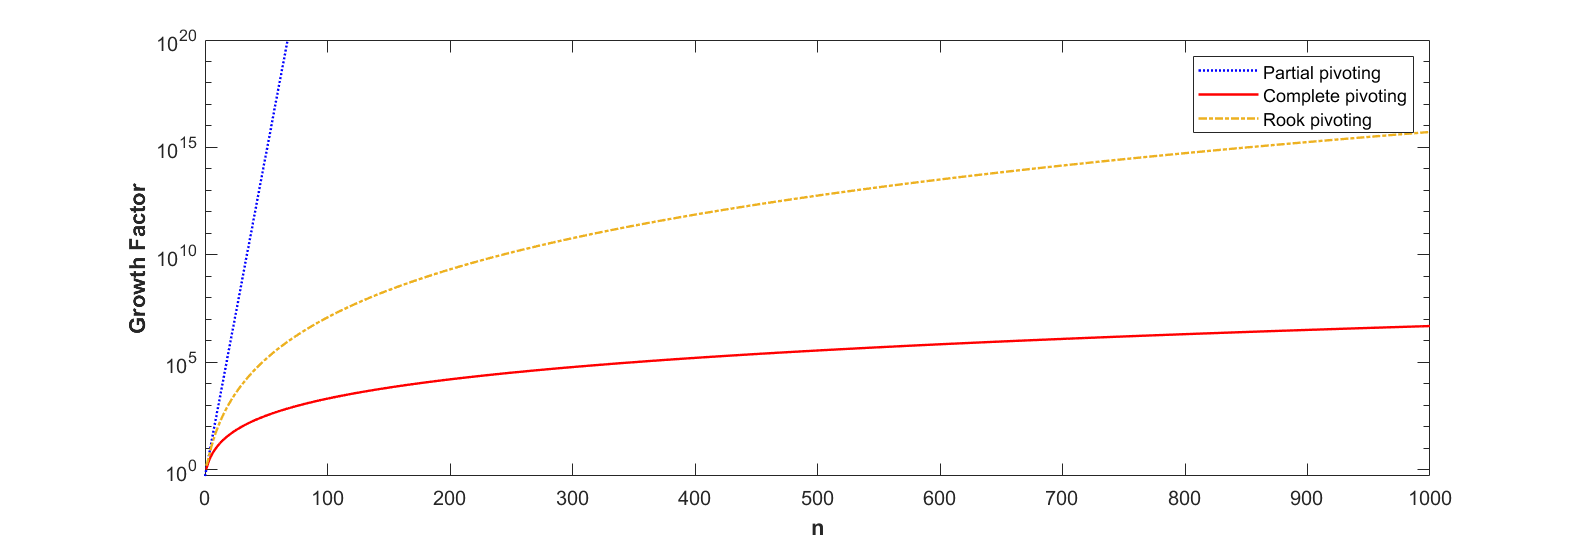
\includegraphics[width=0.8\textwidth]{GrowthFactor.png}
    \caption{三种策略的增长因子上界}\label{fig:GrowthFactor}
\end{figure}

对于一些特殊矩阵,增长因子可以给出足够好的上界。
\subsubsection{对角占优矩阵}
如果矩阵$ A\in \mathbb{C}^{n\times n} $满足
\[
    |a_{ii}| \geqslant \sum_{j\neq i} |a_{ij}|,\quad i=1:n,
\]
则称该矩阵是行对角占优矩阵。类似地,如果
\[
    |a_{ii}| \geqslant \sum_{j\neq i} |a_{ji}|,\quad i=1:n,
\]
则称该矩阵是列对角占优矩阵。如果上述条件中的“$ \geqslant $”变为“$ > $”,则称为强行对角占优或强列对角占优,这类矩阵是非奇异的。很多从有限元方法得到的矩阵都是对角占优的。对行或列对角占优矩阵,我们有如下结论。
\begin{theorem}
    如果$ A $是非奇异的行或列对角占优矩阵,则$ A $的LU分解存在并可以通过GE过程获得,且不选主元的GE增长因子满足
    \begin{equation}
        \rho_n \leqslant 2.
    \end{equation}
    另外,如果$ A $是列对角占优矩阵,则通过GE获得的LU分解中的$ l_{ij}\leqslant 1 $,因此对这类矩阵而言GEPP等价于GE。
\end{theorem}
事实上,根据引理\ref{lem:DiagDom}我们有
\[
    {\rm cond}(U) = \| |U^{-1}| |U| \|_\infty \leqslant 2n-1,
\]
而注意到
\[
    |L| |U| = |A U^{-1}| |U| \leqslant |A| |U^{-1}| |U|,
\]
于是
\[
    \| |L| |U| \|_\infty \leqslant {\rm cond}(U)\| A \|_\infty = (2n-1)\| A \|_\infty.
\]
所以尽管$ L $内的$ m_{ij} $可能很大,但是$ U $内的相应的$ u_{ij} $足够小,使得$ |L| |U| $的大小可以较好地被控制。根据(\ref{eq:GEbackerror}),对一般的矩阵进行GE的后向误差满足
\[
    (A + \Delta A) \hat{x} = b, \quad |\Delta A| \leqslant \gamma_{3n} |\hat{L}| |\hat{U}|
\]
因此对于对角占优矩阵,我们有
\[
    \| \Delta A \|_\infty \leqslant \gamma_{3n} \| |\hat{L}| |\hat{U}| \|_\infty\lesssim (2n-1)\gamma_{3n} \| A \|_\infty,
\]
所以这种情况下原始Gauss消元法是后向稳定的。

\subsubsection{带状矩阵}
\begin{figure}[htpb]
    \centering
    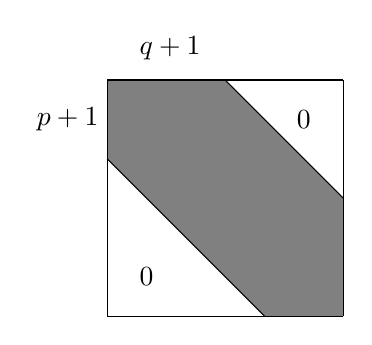
\begin{tikzpicture}
        \fill[gray] (0,2) -- (2,0) -- (3,0) -- (3,1.5) -- (1.5, 3) -- (0,3) -- cycle;
        \draw[-] (0, 0) -- (0, 3);
        \draw[-] (0, 0) -- (3, 0);
        \draw[-] (0, 3) -- (3, 3);
        \draw[-] (3, 0) -- (3, 3);
        \draw[-] (0, 2) -- (2, 0);
        \draw[-] (1.5, 3) -- (3, 1.5);
        \node[] at (2.5, 2.5) {$ 0 $};
        \node[] at (0.5, 0.5) {$ 0 $};
        \node[] at (-0.5, 2.5) {$ p+1 $};
        \node[] at (0.8, 3.4) {$ q+1 $};
      \end{tikzpicture}
    \caption{带状矩阵}
    \label{fig:BandMatrix}
\end{figure}
如图\ref{fig:BandMatrix}所示,如果矩阵$ A\in \mathbb{C}^{n\times n} $满足
\begin{equation}
    a_{ij} = 0, \quad i-j>p \text{ or } j-i>q,
\end{equation}
则称该矩阵是带状矩阵,其中$ p $和$ q $分别称为上带宽和下带宽。对于带状矩阵,我们有如下结论。
\begin{theorem}
    如果$ A $是上下带宽分别为$ p,q $的带状矩阵,则使用GEPP得到的LU分解$ PA = LU $中,$ L $的每列最多有$ p+1 $个非零元,$ U $的上带宽为$ p+q $。并且部分主元的GE增长因子满足
    \begin{equation}
        \rho_n^p \leqslant 2^{2p-1} - (p-1)2^{p-2},
    \end{equation}
    并且右端上界在$ n=2p+1 $时几乎达到。
\end{theorem}

在QR算法中起重要作用的上Hessenberg矩阵($ i-j>1 $时$ a_{ij} = 0 $)是一类特殊的带状矩阵,它在部分主元策略的GE的增长因子满足
\[
    \rho_n^p \leqslant n.
\]

另一类重要的带状矩阵是三对角矩阵,即
\[
    A = 
    \begin{pmatrix}
        d_1 & e_1 & & & \\
        c_2 & d_2 & e_2 & & \\
        & c_3 & d_3 & \ddots & \\
        & & \ddots & \ddots & e_{n-1} \\
        & & & c_{n} & d_n
    \end{pmatrix}.
\]
它的LU分解$ A = LU $形如
\[
    L = 
    \begin{pmatrix}
        1 & & & & \\
        l_2 & 1 & & & \\
        & l_3 & 1 & & \\
        & & \ddots & \ddots & \\
        & & & l_n & 1
    \end{pmatrix},\quad U =
    \begin{pmatrix}
        u_1 & e_1 & & & \\
        & u_2 & e_2 & & \\
        & & \ddots & \ddots & \\
        & & & \ddots & e_{n-1} \\
        & & & &  u_n
    \end{pmatrix},
\]
消元过程简化为$ u_1 = d_1 $,以及
\[
    \begin{aligned}
        l_i &= c_i / u_{i-1},\quad i=2:n,\\
        u_i &= d_i - l_i e_{i-1},\quad i=2:n.
    \end{aligned}
\]
所以计算结果满足
\[
    \begin{aligned}
        (1+\epsilon_i)\hat{l}_i &= c_i / \hat{u}_{i-1},\quad |\epsilon_i|\leqslant u\\
        (1+\theta_i)\hat{u}_i &= d_i - \hat{l}_i e_{i-1}(1+\delta_i),\quad |\theta_i|,|\delta_i|\leqslant u.
    \end{aligned}  
\]
于是
\[
    \begin{aligned}
        |c_i - \hat{l}_i \hat{u}_{i-1}| &\leqslant  u(\hat{l}_i \hat{u}_{i-1}),\\
        |d_i - \hat{u}_i - \hat{l}_ie_{i-1}| &\leqslant  u(|\hat{l}_{i} e_{i-1} +|\hat{u}_{i}|).
    \end{aligned}
\]
即
\begin{equation}
    A - \hat{L} \hat{U} = \Delta A, \quad |\Delta A| \leqslant u|\hat{L}| |\hat{U}|.
\end{equation}
使用回代法计算引入的误差满足
\begin{equation}
    (\hat{L}+\Delta L)(\hat{U} + \Delta U)\hat{x} = b,\quad |\Delta L|\leqslant u|\hat{L}|,|\Delta U| \leqslant (2u+u^2)|\hat{U}|,
\end{equation}
因此最终的后向误差满足
\begin{equation}
    (A+\Delta A)\hat{x} = b,\quad |\Delta A| \leqslant (4u+3u^2+u^3)|\hat{L}| |\hat{U}|.
\end{equation}

有几类特殊的三对角矩阵满足之前的$ |L| |U| = |LU| $的条件,这些矩阵的LU分解的增长因子可以给出较好的上界。
\begin{theorem}
    如果非奇异的三对角矩阵$ A $可以进行LU分解并且满足以下条件之一:
    \begin{enumerate}
        \item $ A $是对称正定的;
        \item $ A $是完全非负的,或等价地存在$ L\geqslant 0,U\geqslant 0 $使得$ A=LU $;
        \item $ A $是M-矩阵,即$ L $和$ U $的对角元都是正的,且非对角元非负;
        \item $ A = D_1BD_2 $,其中$ B $是满足之前条件之一的矩阵,$ |D_1|=|D_2|=I $是符号矩阵;
    \end{enumerate}
    则$ A $的LU分解满足$ |L| |U| = |LU| $。并且当$ A $是以上四类矩阵之一时,如果单位舍入误差$ u $足够小,则Gauss消元得到的数值解$ \hat{x} $满足如下后向误差关系:
    \begin{equation}
        (A+\Delta A)\hat{x} = b,\quad |\Delta A| \leqslant \frac{4u+3u^2+u^3}{1-u}|A|.
    \end{equation}
\end{theorem}

另外,如果矩阵$ A $是三对角矩阵但不属于上述定理中的四类矩阵之一,而只是行或列对角占优的,则虽然此时$ |L| |U| $可能不和$ |LU|=|A| $相同,但是$ |L| |U| $的大小仍然可以被控制,我们有
\[
    |L| |U| \leqslant 3|A|.
\]

\subsection{LU分解的稳定性}
这一节的最后,我们回过来考虑LU分解的敏感性问题,之前已经给出了LU分解的后向误差关系:
\[
    \hat{L} \hat{U} = A + \Delta A,\quad |\Delta A| \leqslant \gamma_{n} |\hat{L}| |\hat{U}|,
\]
但没有给出前向误差估计。尽管对于大多数应用而言,LU分解的前向误差分析不像后向误差分析那样重要,在这里我们还是给出一个简单的前向误差估计(ANSA Th 9.15)。
\begin{theorem}
    如果$ A\in \mathbb{R}^{n\times n} $非奇异,扰动后的$ A+\Delta A $也可逆,并且两者都有LU分解:
    \[
        A = LU, \quad A+\Delta A = (L+\Delta L)(U +\Delta U).
    \]
    令$ G = L^{-1}\Delta A U^{-1} $,则在$ \| G \|_2 $时,LU分解的前向误差满足
    \begin{equation}
        \max\left\{ \frac{\| \Delta L \|_F }{\| L \|_2}, \frac{\| \Delta U \|_F }{\| U \|_2} \right\} 
        \leqslant \frac{\| G \|_F}{1-\| G \|_2}\leqslant 
        \frac{\| L^{-1} \|_2 \| U^{-1} \|_2 \| A \|_2}{1-\| L^{-1} \|_2 \| U^{-1} \|_2 \| \Delta A \|_2} \cdot \frac{\| \Delta A \|_F}{\| A \|_F}.
    \end{equation}
    另外记$ \tilde{G} = (L+\Delta L)^{-1} \Delta A (U+\Delta U)^{-1} $,如果$ |\tilde{G}| $的谱半径(最大绝对值的特征值)小于$ 1 $,则有
    \begin{equation}
        \begin{aligned}
            |\Delta L|&\leqslant |L+\Delta L|\cdot {\rm stril}((I-|\tilde{G}|)^{-1}|\tilde{G}|),\\
            |\Delta U|&\leqslant {\rm triu}(|\tilde{G}|(I-|\tilde{G}|)^{-1}) \cdot |U+\Delta U|,
        \end{aligned}
    \end{equation}
    其中$ {\rm stril}(\cdot) $和$ {\rm triu}(\cdot) $分别表示取矩阵的严格下三角部分和上三角部分。
\end{theorem}

如果记$ \chi(A) = \| L^{-1} \|_2 \| U^{-1} \|_2 \| A \|_2 $,则不难证明
\[
    \kappa_2(A)\leqslant \chi(A)\leqslant \min\{\kappa_2(L), \kappa_2(U)\}\cdot \kappa_2(A).
\]
另外,上述定理的第二部分给出的分量意义下的上界中存在未知的矩阵$ \Delta L $和$ \Delta U $,因此无法直接使用,我们通常令$ \Delta L = \Delta U = 0 $以得到一个与正确上界一阶项相同($ \Delta L, \Delta U\to 0 $时的极限相同)的近似上界。

\section{对称正定矩阵的Cholesky分解}

\subsection{Cholesky分解}

\subsubsection{Cholesky分解的误差分析和稳定性分析}

\subsection{半正定矩阵}

\section{对称矩阵的\texorpdfstring{$ LDL^T $}{LDL-T}分解}

\subsection{分块\texorpdfstring{$ LDL^T $}{LDL-T}分解}

\subsection{Aasen方法}

\section{迭代细化}

\subsection{误差分析}

\subsection{稳定性分析}

\section{分块LU分解}

\bibliography{Lib}
\end{document}